\documentclass[times, 10pt]{thesisMDH}
\usepackage[ddmmyyyy]{datetime}
\usepackage[pdfborder={0 0 0},colorlinks=true,urlcolor=blue,citecolor=red,bookmarks=false]{hyperref}
\usepackage{float}
\usepackage{makecell}
% \usepackage{indentfirst}
\setlength\parindent{0pt}

\university{University of Science and Technology of Hanoi}
\department{Information and Communication Technology}

\subject{Distributed System}
\thesisTitle{Practical Work 5:\\The Longest Path}

\authorOne{Nguyen Phuong Thao}{BI9-212}
\authorTwo{Doan Tuyet Mai}{BI9-162}
\authorThree{Trinh Thao Phuong}{BI9-191}
\authorFour{Phung Kim Son}{BI9-202}
\authorFive{Pham Minh Long}{BI9-146}

\theDate{Hanoi, Mar 2021} 

\begin{document}
\titlePage

\newpage

\mainmatter

\section{How your Mapper and Reducer work?}
\begin{figure}[H]
    \centering
    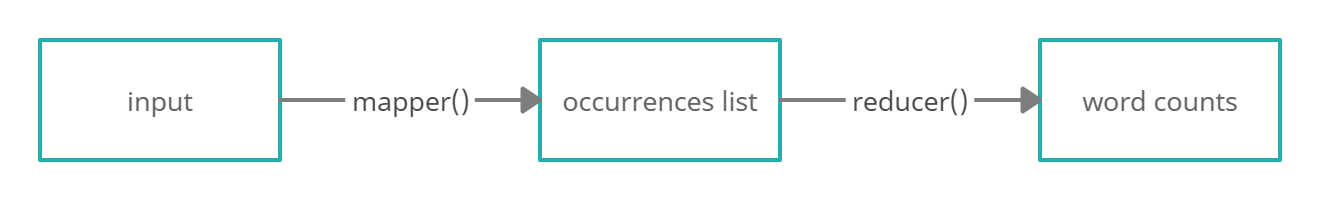
\includegraphics[width=1\linewidth]{images/4-1.png}
    \caption{Mapper and Reducer}
    \label{fig:my_label}
\end{figure}
To generate a list containing the path to files with 20 lines, run this line in the command line:
\begin{lstlisting}
$ sudo find / | head -n 20 > sample.txt
\end{lstlisting}
\subsection{Mapper}
When we received all the paths, we run the \verb|strip()| function to remove the leading and trailing whitespace if there any of it. After that, we split the sentences into words with separator is "\backslash".

\begin{lstlisting}
def mapper(line):
	occurence = []

	line = line.strip()
	f_dir = line.split("/")
	f_dir = filter(None, f_dir)
				
	for d in f_dir:
		occurence.append([d, 1])

	return occurence
\end{lstlisting}
\subsection{Reducer}
After get the words which are the results of the mapper process, we count the number of each words in a path and return the total number of each path. The one with the highest count number will be the longest path.
\begin{lstlisting}
def reducer(occurence):
	path = ""
	count = 0

	for i in range(len(occurence)):
		path = path + occurence[i][0] + "/"
		count = count + occurence[i][1]

	return {path: count}
\end{lstlisting}
\section{Contribution}
\begin{center}
    \begin{tabular}{|l|l|l|}
        \hline
        \textbf{Student} & \textbf{Student ID} & \textbf{Contribution}\\
        \hline
        Pham Minh Long & BI9-146 & Write report\\
        \hline
        Phung Kim Son & BI9-202 & Research for different MapReduce implementation\\
        \hline
        Trinh Thao Phuong & BI9-191 & Draw figures, briefly description \\
        \hline
        Doan Tuyet Mai & BI9-162 & Implement code for Longest Path (MapReduce) \\
        \hline
        Nguyen Phuong Thao & BI9-212 & Explanation of map reduce\\
        \hline
    \end{tabular}
\end{center}

\end{document}
